\newpage

\section{Der Leader}
Die \gls{CPU} bildet das Herzstück eines Computers. Sie ist zuständig, um verschiedene Instruktionen auszuführen. Wenn
z.B. zwei Zahlen addiert werden sollen, dann ist die CPU das Stück Hardware, welches diese Arbeit erledigt.\par
\begin{minipage}{\linewidth}
    \centering
    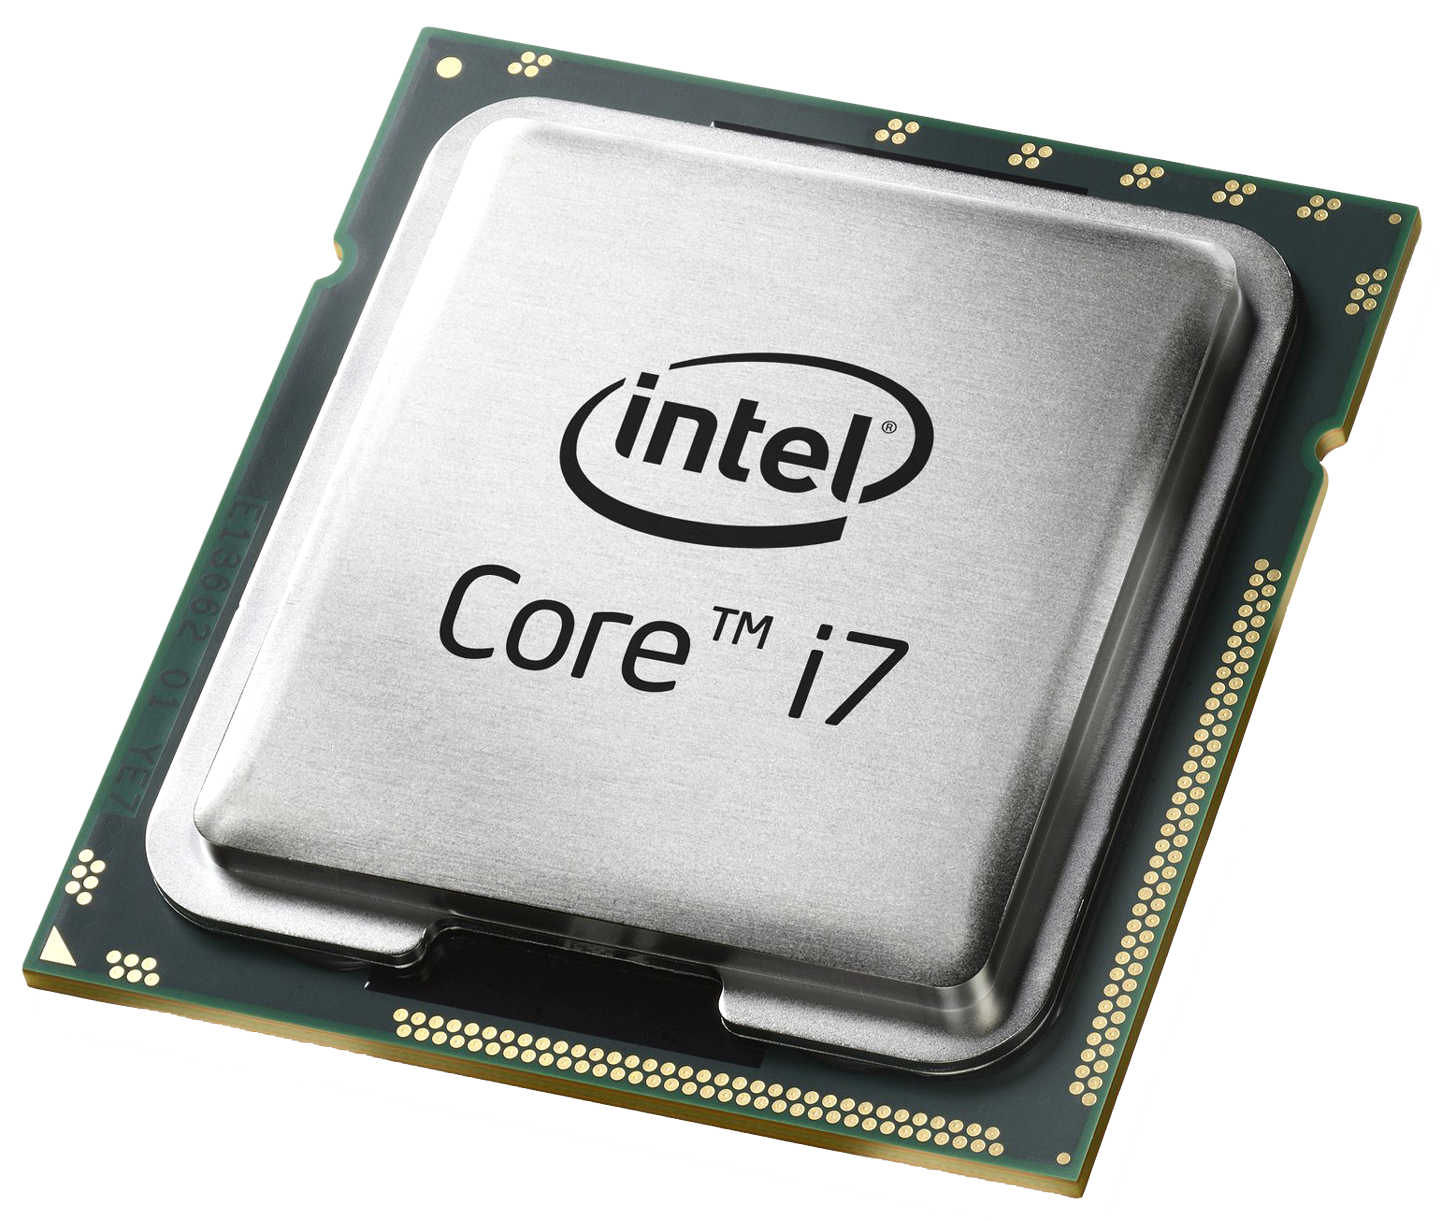
\includegraphics[width=0.2\textwidth]{../common/chapter_02/resources/01_cpu_intel.png}
    \captionof{figure}{Intel CPU}
\end{minipage}
Nun fragt man sich zurecht, wie die CPU denn solche Aufgaben bewältigen kann? Dazu muss man wissen, dass die CPU
selbst wiederum aus mehreren Teilen besteht, die alle eine bestimmte Aufgabe erfüllen. Es sind dies im Wesentlichen:
\begin{description}
    \item[Control unit] Diese Einheit steuert den ganzen Ablauf der CPU. Sie sagt den anderen Komponenten im Gerät und
    in der CPU selbst, was sie wann tun sollen und steuert so den ganzen Computer.\cite{wikipedia:cu}
    \item[Arithmetic logic unit] Wenn arithmetische oder logische Operationen durchgeführt werden sollen, dann ist diese
    Einheit wichtig. Wenn z.B. 4 + 5 gerechnet werden soll, dann wird die \gls{ALU} damit beauftragt.\cite{wikipedia:alu}
    \item[Address generation unit] Will die CPU auf den Hauptspeicher (RAM) zugreifen, dann wird in dieser Einheit die korrekte
    Adresse berechnet. Was das genau bedeutet wird im nächsten Abschnitt erklärt.\cite{wikipedia:agu}
\end{description}
Die CPU beinhaltet noch mehr solcher Einheiten, auf diese wird aber nun nicht mehr weiter eingegangen.

\subsection{Übung 1 - Computer und Zahlen}
Es wird Zeit für die erste kleine Übung. Wir wollen darin das Verständnis stärken, wie Zahlen überhaupt in einem Computer
dargestellt werden und wie wir in der Lage sind, diese zu addieren.\\
Du hast sicher schon gehört, dass ein Computer mit 1en und 0en arbeitet. Wir wollen uns nun anschauen, was das genau bedeutet.\\
Dazu musst du dir aber erst mal darüber klar werden, wie wir Menschen uns Zahlen vorstellen, respektive, wie wie wir
sie darstellen.\\
Wie ihr wohl sicherlich auch bereits gehört habt, arbeiten wir mit dem 10er-System. Das bedeutet nichts anderes, als dass
wir zehn verschiedene Ziffern kennen, um eine Zahl darzustellen. In dem Fall 0 bis 9.\\
Nehmen wir nun als Beispiel die Zahl $145$.
Natürlicherweise interpretieren wir diese Zahl korrekt, wir machen uns aber nicht
wirklich über den Aufbau an sich Gedanken. Wir wollen nun diese Zahl ein wenig anders formulieren und sie zuerst einmal
auseinander nehmen. Dabei hilft uns das Wissen weiter, dass wir uns im 10er-System befinden (Basis 10).\\
Analysieren wir nun zuerst einmal unsere Zahl. Darin gibt es eine 1, diese steht ganz links an dritter Stelle. Sie bildet die Wertigkeit 100.
Die zweite Ziffer ist eine  4, sie steht in der Mitte an zweiter Stelle und bildet die Wertigkeit 10. Die dritte Ziffer steht ganz rechts an erster Stelle
und bildet die Wertigkeit 1.\\\\
Ausgangslage dieser Zahl ist nun erstmal die Ziffer 1.\\
Die Frage stellt sich jetzt, wie wir die 1 an die Stelle ganz links verschieben können. Ganz konkret stellen wir uns die
Frage, wie wir aus der Zahl 1 die Zahl 100 machen?\\
Wir haben dazu das Werkzeug der Multiplikation und können z.B. die 1 einfach mit der entsprechenden Wertigeit multiplizieren, wohin
wir die Ziffer verschieben wollen. In dem Fall ist es die Wertigkeit 100:\\
$1 \times 100 = 100$\\
\begin{exerciseseries}[columns=1,solsubrule=\hrule]{}
    \begin{exercise}
        Überlege dir kurz, wie wir die 4 an die Position in der Mitte verschieben können:\\
        $4 \times $\underline{\hspace{1cm}} $ = 40$
    \end{exercise}
    \begin{solution}
        $4 \times 10 = 40$
    \end{solution}

    \begin{exercise}
        Und nun überlege dir, was wir mit der 5 ganz rechts machen müssen?\\
        $5 \times $\underline{\hspace{1cm}} $ = 5$
    \end{exercise}
    \begin{solution}
        $5 \times 1 = 5$
    \end{solution}
\end{exerciseseries}

Sobald wir alle Ziffern korrekt verschoben haben, ergibt sich das folgende Bild:

\begin{alignat*}{3}
    1 \times && 100 = && 100\\
    4 \times && 10 = && 40\\
    5 \times && 1 = && 5
\end{alignat*}

Wir stellen uns einmal mehr die Frage, wie wir nun aus diesen Einzelteilen unsere Zahl 145 erhalten?\\
Die Lösung ist in dem Fall in der Form der Addition gegeben. Sobald die Ziffern an die jeweils richtigen Positionen
verschoben wurden, können wir diese einfach alle aufsummieren (addieren).

\begin{alignat*}{1}
    100 + 40 + 5 = 145
\end{alignat*}

So weit, so gut. Wir merken uns:
\begin{itemize}
    \item Zuerst verschieben wir die Ziffern alle mittels Multiplikation an die korrekte Position.
    \item Danach setzen wir die Zahl aus den einzelnen Resultaten mithilfe der Addition zusammen.
\end{itemize}

Nun wollen wir aber eigentlich nur noch mit der Basis 10 arbeiten. Das bedeutet, wir wollen bei der Multiplikation nicht
die Wertigkeit an sich verwenden, sondern diese durch die Basis ausdrücken. Dazu müssen wir uns aber zuerst einmal in
Erinnerung rufen, was ein Exponent ist. Diese kleinen Gleichungen sollte ein wenig Licht ins Dunkel bringen.\\
$m \times m = m^2$\\
$10 \times 10 = 10^2$\\
$2 \times 2 \times 2 = 2^3$\\
\newpage
Mache dir dazu ein paar Gedanken und versuche die folgenden Übungen auszufüllen. Schreibe wenn möglich die Lösung
mit Exponenten.
\begin{exerciseseries}[columns=2,solsubrule=\hrule]{}
    \begin{exercise}
        $10 \times 10 = $\underline{\hspace{1cm}}
    \end{exercise}
    \begin{solution}
        $10 \times 10 = 10^2 = 100$
    \end{solution}

    \begin{exercise}
        $10 \times 10 \times 10 = $\underline{\hspace{1cm}}
    \end{exercise}
    \begin{solution}
        $10 \times 10 \times 10 = 10^3 = 1000$
    \end{solution}

    \begin{exercise}
        $10 \times 5 = $\underline{\hspace{1cm}}
    \end{exercise}
    \begin{solution}
        $10 \times 5 = 50$
    \end{solution}

    \begin{exercise}
        $10^x = 1 \Rightarrow x = $\underline{\hspace{1cm}}
    \end{exercise}
    \begin{solution}
        $10^0 = 1 \Leftrightarrow \{10^x = 1 \Rightarrow x = 0\}$
    \end{solution}
\end{exerciseseries}

Da wir uns nun auch die Exponenten wieder in Erinnerung gerufen haben, können wir dieses Umhergeschiebe der Ziffern
nun auch elegant mit der Basis ausdrücken.
\begin{alignat*}{3}
    1 \times && 10^2 = && 100\\
    4 \times && 10^1 = && 40\\
    5 \times && 10^0 = && 5
\end{alignat*}
Das ganze können wir nun noch in Tabellenform überführen. In der ersten Zeile steht jeweils die Wertigkeit, in der
zweiten Zeile der Faktor (die zu verschiebende Ziffer).\\
\begin{center}
    \begin{tabular}{ c c c c }
        Wertigkeit & $10^2$ & $10^1$ & $10^0$ \\
        Faktor     & $1$    & $4$    & $5$
    \end{tabular}
\end{center}

Nun sind wir definitiv bereit, den nächsten Schritt zu tun. Wir wollen uns einige Gedanken zur Basis machen. Bis jetzt
haben wir in unserem bekannten natürlichen Umfeld der Basis 10 gearbeitet. Der Computer hat aber eine kleine technische
Einschränkung. Er arbeitet mit Strom. Er kennt also nur den Zustand \frqq ich habe eine Ladung\flqq{} und den Zustand \frqq ich habe
keine Ladung\flqq. Wie wir richtig bemerkt haben, handelt es sich hierbei um ein binäres System, wir kennen also im Gegensatz
zu unserem 10er-System nur zwei Zustände (0 und 1).\footnote{Ein kleiner Exkurs: Die Darstellung der Ziffer in einem System spielt eigentlich keine Rolle.
Wir könnten für die Zustände auch a und b verwenden. Wenn du dich dafür interessierst, dann schaue dir mal das \frqq Martian number system\flqq{} an.
Suche entweder bei Google danach oder nütze folgenden link \url{https://mathematicscentre.com/taskcentre/098martn.htm}. Zu unseren Übungen gibt es
auch noch eine gute Website, die vielleicht das eine oder andere noch ein wenig besser erklärt \url{https://www.freecodecamp.org/news/martian-math-812a029e2ea0/}}\\
Von diesem Moment an arbeiten wir also nur noch mit 0 und 1. Wir können die Ziffern 2 bis 9 nicht mehr verwenden, da diese
gar nicht mehr existieren. Jetzt fragen wir uns natürlich zurecht, wie wir denn unsere 145 ausdrücken sollen ohne die 4 und die 5?\\
Dazu versuchen wir uns erst an einer anderen Zahl, nämlich einer Binären. Diese Zahl sieht nun folgendermassen aus:\\
$10011$\\
Nun denn, wir machen uns auch hier ein wenig mehr Gedanken über den Aufbau der Zahl. Wir erkennen, dass auch hier ganz
links aussen eine 1 steht. Nun wissen wir bereits, wie wir im 10er-System eine Ziffer auf die richtige Position verschieben
können. Glücklicherweise funktioniert dies hier genau gleich, es gibt nur einen Unterschied und zwar die Basis.

\newpage
\begin{exerciseseries}[columns=1,solsubrule=\hrule]{}
    Folgende Positionen sind innerhalb der Zahl gegeben:
    \begin{center}
        \begin{tabular}{ c c c c c c }
            Position & $5$ & $4$ & $3$ & $2$ & $1$ \\
            Ziffer & $1$ & $0$ & $0$ & $1$ & $1$
        \end{tabular}
    \end{center}
    \begin{exercise}
        Verschiebe die Ziffer '1' an die Position 5 im 10er System.\\
        \underline{\hspace{12cm}}
    \end{exercise}
    \begin{solution}
        $1 * 10^4 = 10000$
    \end{solution}

    \begin{exercise}
        Verschiebe die Ziffer '1' an die Position 5 im 2er System.\\
        \underline{\hspace{12cm}}
    \end{exercise}
    \begin{solution}
        $1 * 2^4 = 10000$
    \end{solution}

    \begin{exercise}
        Verschiebe die Ziffer '0' an die Position 4 im 2er System.\\
        \underline{\hspace{12cm}}
    \end{exercise}
    \begin{solution}
        $0 * 2^3 = 0000$
    \end{solution}

    \begin{exercise}
        Verschiebe die Ziffer '0' an die Position 3 im 2er System.\\
        \underline{\hspace{12cm}}
    \end{exercise}
    \begin{solution}
        $0 * 2^2 = 000$
    \end{solution}

    \begin{exercise}
        Verschiebe die Ziffer '1' an die Position 2 im 2er System.\\
        \underline{\hspace{12cm}}
    \end{exercise}
    \begin{solution}
        $1 * 2^1 = 10$
    \end{solution}

    \begin{exercise}
        Verschiebe die Ziffer '1' an die Position 1 im 2er System.\\
        \underline{\hspace{12cm}}
    \end{exercise}
    \begin{solution}
        $1 * 2^0 = 1$
    \end{solution}
\end{exerciseseries}

Wenn du mit den Übungen durch bist, hast du wahrscheinlich schon erkannt, dass du die Bestandteile der Zahl 10011 im binären
System korrekt aufgebaut hast.
\begin{alignat*}{3}
    1 \times && 2^4 = && 10000\\
    0 \times && 2^3 = &&  0000\\
    0 \times && 2^2 = &&   000 \\
    1 \times && 2^1 = &&    10 \\
    1 \times && 2^0 = &&     1 \\
\end{alignat*}

Wie im 10er-System auch erhalten wir hier die fertige Zahl über das Werkzeug \frqq Addition\flqq.
\begin{alignat*}{1}
    10000 + 0000 + 000 + 10 + 1 = 10011
\end{alignat*}
Nun ist euch wahrscheinlich schon aufgefallen, dass die folgende Rechnung im 10er-System natürlich auch eine Lösung hat.
\begin{alignat}{2}
    1 \times 2^4 = && (10000)_2\\
    1 \times 2^4 = && (16)_{10}
\end{alignat}
Die Zeile 2.1 beinhaltet das Resultat dargestellt im binären System mit 0 und 1. Siehe dazu die kleine 2 hinter der Klammer.\\
Die Zeile 2.2 beinhaltet das Resultat dargestellt im 10er-System mit den Ziffern 0 bis 9. Siehe dazu die kleine 10 hinter der Klammer.
Und genau so funktioniert tatsächlich die Umrechnung von jedem beliebigen System ins 10er-System.
Das bedeutet, dass die Zahl 10000 im binären der Zahl 16 im 10er-System entspricht.
\begin{exerciseseries}[columns=1,solsubrule=\hrule]{}
    \begin{exercise}
        Ok, soweit so gut. Was ist jetzt aber mit der Zahl $(11)_2$ im Binären? Wie können wir so eine Zahl ins 10er-System umrechnen?\\
        Mache dir dazu ein paar Gedanken und schreibe mal auf, wie du vorgehen würdest. Wenn du denkst, dass du entweder die Lösung gefunden
        hast oder du nicht mehr weiterweist, dann wirf auf jeden Fall einen Blick in die Lösungen. Dort wird der Vorgang nochmals ausführlich
        anhand eines Beispiels erklärt.\\
        \underline{\hspace{15cm}}
        \underline{\hspace{15cm}}
        \underline{\hspace{15cm}}
        \underline{\hspace{15cm}}
        \underline{\hspace{15cm}}
        \underline{\hspace{15cm}}
        \underline{\hspace{15cm}}
        \underline{\hspace{15cm}}
        \underline{\hspace{15cm}}
        \underline{\hspace{15cm}}
    \end{exercise}
    \begin{solution}
        Um die Zahl $(11)_2$ ins 10er-System zu überführen, betrachten wird die Zahl zuerst einmal wieder über ihre Bestandteile.\\
        Wir nehmen sie also auseinander, wie wir das auch schon kennen.\\
        \begin{alignat*}{3}
            1 \times && 2^1 = &&    (10)_2, (2)_{10} \\
            1 \times && 2^0 = &&     (1)_2, (1)_{10} \\
        \end{alignat*}
        Und wie wir auch schon wissen, können wir über die Addition die Zahlen wieder zusammenfügen. Dies tun wir nun ebenfalls:
        \begin{alignat*}{1}
            (10)_2 + (1)_2 = (11)_2 \\
            (2)_{10} + (1)_{10} = (3)_{10}
        \end{alignat*}
        Nun könnt ihr erkennen, dass die Lösung im binären System wieder die Ausgangszahl ergibt, wenn wir die Zahl aber
        im 10er-System interpretieren, dann ergibt dies uns 3, was genau der Zahl 11 im binären entspricht. Wir merken
        uns also:\\
        Wir können eine Zahl in einer anderen Basis als 10 ganz einfach ins 10er-System überführen, wenn wir die Zahl
        in ihren Bestandteilen betrachten und die jeweilige Ziffer an dieser Position mit ihrer Wertigkeit multiplizieren.
        Haben wir das getan, so können wir über die Addition die Zahl wieder zusammensetzen.
    \end{solution}
    \begin{exercise}
        Rechne die folgende Zahl ins 10er-System um: $(100)_2$\\
        \underline{\hspace{12cm}}
    \end{exercise}
    \begin{solution}
        $1 \times 2^2 + 0 \times 2^1 + 0 \times 2^0 = 4$
    \end{solution}

    \begin{exercise}
        Rechne die folgende Zahl ins 10er-System um: $(101)_2$\\
        \underline{\hspace{12cm}}
    \end{exercise}
    \begin{solution}
        $1 \times 2^2 + 0 \times 2^1 + 1 \times 2^0 = 5$
    \end{solution}

    \begin{exercise}
        Rechne die folgende Zahl ins 10er-System um: $(10010001)_2$\\
        \underline{\hspace{12cm}}
    \end{exercise}
    \begin{solution}
        $1 \times 2^7 + 0 \times 2^6 + 0 \times 2^5 + 1 \times 2^4 + 0 \times 2^3 + 0 \times 2^2 + 0 \times 2^1 + 1 \times 2^0 = 145$
    \end{solution}

    \begin{exercise}
        Rechne die folgende Zahl ins 10er-System um: $(100)_3$\\
        \underline{\hspace{12cm}}
    \end{exercise}
    \begin{solution}
        $1 \times 3^2 + 0 \times 3^1 + 0 \times 3^0 = 9$
    \end{solution}
\end{exerciseseries}
Wir haben nun also gesehen, wie wir Zahlen interpretieren und in anderen Systemen darstellen können. Weiterhin sind wir
in der Lage von jedem beliebigen System aus ins 10er-System zu konvertieren.

\newpage
\subsection{\solutionsname}
\loadSolutions
\subsection{Übung 2 - Einmal mehr eine Addition}
Wir wollen nun noch einen Schritt weitergehen  und uns einen Teil der Arbeit der \gls{ALU} anschauen,
nämlich die Addition zweier Zahlen im binären System. Um den Einstieg zu vereinfachen, wollen wir uns zuerst mit
etwas auseinandersetzen, das wir bereits in der Unterstufe gelernt haben. Die schriftliche Addition im 10er-System.\\
Weisst du noch, wie das geht?\\
\begin{exerciseseries}[columns=1,solsubrule=\hrule]{}
    \begin{exercise}
        Addiere die Zahlen 25 und 2 schriftlich. Wenn du nicht mehr weisst, wie das geht, dann schaue in den Lösungen.
        \vspace{5cm}
    \end{exercise}
    \begin{solution}
        \opadd[carryadd=true,lastcarry]{25}{2}
    \end{solution}
    \begin{exercise}
        Addiere die Zahlen 25 und 7.
        \vspace{5cm}
    \end{exercise}
    \begin{solution}
        \opadd[carryadd=true,lastcarry]{25}{7}
    \end{solution}
    \begin{exercise}
        Addiere die Zahlen 99 und 99.
        \vspace{5cm}
    \end{exercise}
    \begin{solution}
        \opadd[carryadd=true,lastcarry]{99}{99}
    \end{solution}
    \begin{exercise}
        Addiere die Zahlen 45 und 72.
        \vspace{5cm}
    \end{exercise}
    \begin{solution}
        \opadd[carryadd=true,lastcarry]{45}{72}
    \end{solution}
\end{exerciseseries}
\newpage
Da wir jetzt ein wenig repetiert haben, können wir uns etwas Neuem widmen. Wir machen jetzt genau dasselbe, nur
im binären System.

\begin{exerciseseries}[columns=1,solsubrule=\hrule]{}
    \begin{exercise}
        Addiere die Zahlen 2 $(10)_2$ und 1 $(1)_2$ schriftlich im Binärsystem.
        \vspace{5cm}
    \end{exercise}
    \begin{solution}
        \opaddbin{2}{1}{}
    \end{solution}
    \begin{exercise}
        Addiere die Zahlen 3 $(11)_2$ und 1 $(1)_2$ schriftlich im Binärsystem.
        \vspace{5cm}
    \end{exercise}
    \begin{solution}
        \opaddbin{3}{1}{6}
    \end{solution}
    \begin{exercise}
        Addiere die Zahlen 12 $(1100)_2$ und 22 $(10110)_2$ schriftlich im Binärsystem.
        \vspace{5cm}
    \end{exercise}
    \begin{solution}
        \opaddbin{12}{22}{56}
    \end{solution}
\end{exerciseseries}

\newpage
\subsection{\solutionsname}
\loadSolutions
\newpage
\subsection{Übung 3 - Logische Operationen}
Was uns jetzt noch fehlt ist das Verständnis von logischen Operationen. Es geht im Grunde nur darum,
zwei Bedingungen auszuwerten und auf einen Wahrheitswert zu überführen. Nehmen wir als Beispiel einmal an,
dass wir die folgenden Aussagen haben:
\begin{description}
    \item[Aussage A] Ein Flugzeug ist zum Tauchen gebaut worden.
    \item[Aussage B] 9 ist durch 3 teilbar.
    \item[Aussage C] 5 ist eine Primzahl.
    \item[Aussage D] YB gewinnt in der nächsten Saison die Championsleague.
\end{description}
Wir haben offensichtlich zwei Aussagen (B und C), die der Wahrheit entsprechen und eine
Aussage (A), die nicht zutrifft. Weiterhin gibt es eine Aussage (D), bei der wir den Wahrheitswert nur
erahnen können, aber nicht genau kennen. Doch wir können festhalten, dass in der klassischen Aussagenlogik
eine Aussage also entweder wahr oder falsch sein kann.\cite{wikipedia:aussagenlogik}\\

Wir können diese Aussage nun verknüpfen und daraus eine Neue generieren. Dazu schauen wir uns zwei
Werkzeuge an:
\begin{itemize}
    \item AND (Und) $\land$
    \item OR (Oder) $\lor$
\end{itemize}
Angenommen, wir setzen die Aussagen B und C mithilfe des logischen AND zusammen, dann
lautet die neue Aussage:\\$B \land C$\glqq 9 ist durch 3 teilbar UND 5 ist eine Primzahl\flqq\\
Diese Aussage ist ebenfalls wahr.

\begin{exerciseseries}[columns=1,solsubrule=\hrule]{}
    Wir wollen nun mithilfe dieser Verknüpfungen ein paar Aussagen zusammensetzen. Kreuze das korrekte Resultat an.
    \begin{exercise}
        $A \land B$\\
        Wahr $\square$ \hspace{1cm} Falsch $\square$
    \end{exercise}
    \begin{solution}
        Wahr $\square$ \hspace{1cm} Falsch $\boxtimes$
    \end{solution}

    \begin{exercise}
        $A \lor B$\\
        Wahr $\square$ \hspace{1cm} Falsch $\square$
    \end{exercise}
    \begin{solution}
        Wahr $\boxtimes$ \hspace{1cm} Falsch $\square$
    \end{solution}

    \begin{exercise}
        $B \lor C$\\
        Wahr $\square$ \hspace{1cm} Falsch $\square$
    \end{exercise}
    \begin{solution}
        Wahr $\boxtimes$ \hspace{1cm} Falsch $\square$
    \end{solution}
\end{exerciseseries}

\newpage
Zuletzt wollen wir uns noch kurz ansehen, wie wir diese Operationen auch auf binären Zahlen durchführen können
und wie das Resultat aussieht. Dazu betrachten wir uns folgenden Zahlen, welche nun eine Aussage darstellen.
\begin{description}
    \item[Aussage A] 1101 $(13)_{10}$
    \item[Aussage B] 1111 $(15)_{10}$
\end{description}
Um diese Operation nun korrekt durchführen zu können, brauchen wir eine Wahrheitstabelle, um nachschauen zu können,
was bei bestimmten Kombinationen passiert.\\
Die Warheitstabelle für ein logisches AND sieht folgendermassen aus.
\[
    \begin{array}{c | c c}
        \land & 0 & 1 \\ \hline
        0 & 0 & 0 \\
        1 & 0 & 1 \\
    \end{array}
\]
Die Warheitstabelle für ein logisches OR sieht folgendermassen aus.
\[
    \begin{array}{c | c c}
        \lor & 0 & 1 \\ \hline
        0 & 0 & 1 \\
        1 & 1 & 1 \\
    \end{array}
\]
Wir führen nun ein logisches AND auf der Aussage A und B durch.
Dies sieht folgendermassen aus:
\opandbin{13}{15}{13}
Das Resultat dieser Operation ist also wieder 1101 $(13)_{10}$.
\newpage
\begin{exerciseseries}[columns=1,solsubrule=\hrule]{}
    Führe folgende logischen Operationen durch und bestimme auch gleich die Zahl im Zehnersystem.
    \begin{exercise}
        $11001 \land 00110$\\
        \vspace{5cm}
    \end{exercise}
    \begin{solution}
        \opandbin{25}{6}{0}
        Dies entspricht $(0)_{10}$.
    \end{solution}

    \begin{exercise}
        $11001 \lor 00110$\\
        \vspace{5cm}
    \end{exercise}
    \begin{solution}
        \opandbin{25}{6}{31}
        Dies entspricht $(31)_{10}$.
    \end{solution}

    \begin{exercise}
        $1111 \land 0110$\\
        \vspace{5cm}
    \end{exercise}
    \begin{solution}
        \opandbin{15}{6}{6}
        Dies entspricht $(6)_{10}$.
    \end{solution}
\end{exerciseseries}

\newpage
\subsection{\solutionsname}
\loadSolutions

\newpage